
% !TEX encoding = UTF-8 Unicode 
% !TEX root = FieldGuide.tex

\Sec{Exponential Distribution}
\label{sec:Exp}
\dist{Exponential} (Pearson type X, waiting time, negative exponential, inverse exponential) distribution~\cite{Pearson1916,Kondo1930,Johnson1994}:
%
\begin{align}
\label{Exp}
\opr{Exp}(x \given a, \theta) 
= & \frac{1}{|\theta|} \exp\left\{-\frac{x-a}{\theta}\right\} 	\checked
\\ \notag 
& a,\ \theta, \text{ in } \mathbb{R}  					\checked
\\ \notag
\text{support } & x > a, \quad \theta>0 				\checked
\\ \notag
& x < a, \quad \theta<0 							\checked
\end{align}
An important property of the exponential distribution is that it is memoryless\index{memoryless}: assuming positive scale and zero location ($a=0,\ \theta>0$) the conditional probability given that $x>c$, where $c$ is a positive content, is again an exponential distribution with the same scale parameter. The only other distribution with this property is the geometric distribution\index{geometric distribution}, the discrete analog of the exponential distribution. The exponential is the maximum entropy distribution given the mean and semi-infinite support. 



% !TEX encoding = UTF-8 Unicode 
% !TEX root = FieldGuide.tex

\begin{table*}[t!]
\caption[Exponential distribution -- Properties]{Properties of the exponential distribution}
\begin{align*}
\text{\hyperref[PropertiesSec]{Properties}}  \quad& \\
\text{notation} \quad & \op{Exp}(x\given a,\theta)					\checked
\\
\text{PDF}\quad &    \frac{1}{|\theta|} \exp\Left\{-\frac{x-a}{\theta}\Right\} 	\checked
\\
\text{CDF}\big  / \text{CCDF}  \quad  &   1- \exp\Left\{-\frac{x-a}{\theta}\Right\} & \theta>0 \ \big{/} \  \theta<0
\checked
\\
\text{parameters}\quad &   a,\ \theta, \text{ in } \Real 				\checked
\\
\text{support} \quad &   [ a, +\infty]      & \theta>0					\checked
\\
				&   [-\infty,  a]     & \theta <0					\checked
\\
\text{median} \quad  &  a + \theta \ln 2							\checked
\\
\text{mode} \quad  & a										\checked
\\
\text{mean} \quad  &  a+ \theta									\checked						
\\
\text{variance} \quad  & \theta^2								\checked
\\
\text{skew} \quad  &  2										\checked
\\
\text{ex. kurtosis} \quad  &  6										\checked
\\
\text{entropy} \quad  & 1 + \ln |\theta|							\checked
\\
\text{MGF} \quad  & \frac{\exp(at) }{ \Left(1- \theta t\Right)}				\checked
\\
\text{CF} \quad  & \frac{\exp(iat) }{ \Left(1- i \theta t\Right)}				\checked
\end{align*}
\end{table*}



\SSec{Special cases}
\phantomsection\addcontentsline{toc}{subsection}{~~~~~~~~~~~~Anchored exponential}
\phantomsection\addcontentsline{toc}{subsection}{~~~~~~~~~~~~Standard exponential}
The exponential distribution is commonly defined with zero location and positive scale ({\bf anchored exponential}).
With $a=0$ and $\theta=1$ we obtain the {\bf standard exponential} distribution. 

\begin{figure}[tb]
\begin{center}
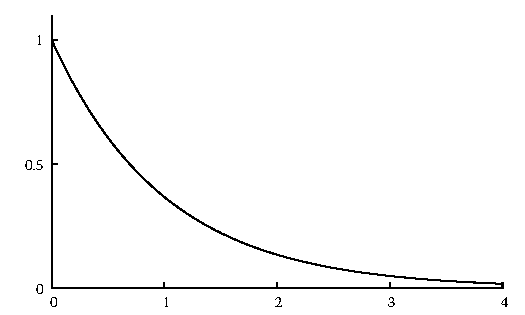
\includegraphics[width=\textwidth]{pdfStdExp}
\end{center}
\caption[Standard exponential distribution]{Standard exponential distribution, $\opr{Exp}(x\given 0,1)$}
\end{figure}


\SSec{Interrelations}

The exponential distribution is common limit of many distributions.
\begin{align*}
	\opr{Exp} (x\given a,\theta)  
	 &	=  \opr{Amoroso}(x\given  a ,\theta,1,1) 	\checked
\\&		\qquad= \opr{Gamma}(x \given a , \theta, 1)	\checked
\\	\opr{Exp} (x\given 0,\theta)  &	=  \opr{Amoroso}(x\given  0 ,\theta,1,1) \checked
 \\ & \qquad =  \opr{Gamma}(x\given  0, \theta,1)  \checked
\\
\opr{Exp}(x\given a,\theta) &=  \lim_{\beta\rightarrow\infty} \opr{PowerFn} (x\given a-\beta\theta,\beta\theta,\beta) 
\checked
\end{align*}

The sum of independent exponentials is an Erlang distribution, a special case of the gamma distribution~\eqref{Gamma}.
\[
\sum_{i=1}^{n} \opr{Exp}_i(0,\theta) \sim \opr{Gamma}(0, \theta, n) \checked
\notag
\]


The minima of a collection of exponentials, with positive scales $\theta_i>0$, is  also exponential,
\[
\op{min}\bigl( \opr{Exp}_1(0,\theta_1),\ \opr{Exp}_2(0,\theta_2),\ \ldots\ ,\ \opr{Exp}_n(0,\theta_n) \bigr) \sim \opr{Exp}(0, \theta') \, , \checked
\notag
\]
where $\theta' = (\sum_{i=1}^{n} \tfrac{1}{\theta_i})^{-1}$. \checked


The order statistics \secref{OrderStatistic} of the exponential distribution are the beta-exponential distribution~\eqref{BetaExp}.
\begin{align*}
\opr{OrderStatistic}&_{\opr{Exp}(\pLoc,\pScale)}  (x \given \alpha, \gamma) =  \opr{BetaExp}(x\given \pLoc, \pScale, \alpha, \gamma)  \checked
\notag
\end{align*}


A Weibull transform of the standard exponential distribution yields the Weibull distribution  \eqref{Weibull}.
\[
\opr{Weibull}(a,\theta,\beta) \sim a+ \theta\ \oprr{StdExp}{Exp}()^{\tfrac{1}{\beta}} \checked
\notag
\]


The ratio of independent anchored exponential distributions is the exponential ratio distribution \eqref{ExpRatio}, a special case of the beta prime distribution \eqref{BetaPrime}.
\label{sec:ExpRatio}
\[
\opr{BetaPrime}(0,\tfrac{\theta_1}{\theta_2} , 1,1) \sim \opr{ExpRatio}(0,\tfrac{\theta_1}{\theta_2}) \sim \frac{\opr{Exp}_1(0,\theta_1)}{\opr{Exp}_2(0,\theta_2) }
\notag
\]

